\documentclass[10pt,a4paper]{article}
\usepackage[utf8]{inputenc}
\usepackage{amsmath}
\usepackage{amsfonts}
\usepackage{amsthm}
\usepackage{amssymb}
\usepackage{caption}
\usepackage{mathtools}
\DeclarePairedDelimiter\Floor\lfloor\rfloor
\DeclarePairedDelimiter\Ceil\lceil\rceil
\usepackage{listings}
\usepackage{color}
\definecolor{light-gray}{gray}{0.92}
\usepackage{graphicx}
\usepackage[left=2cm,right=2cm,top=2cm,bottom=2cm]{geometry}
\usepackage{relsize}
\usepackage[english]{babel}
\usepackage[utf8]{inputenc}
\usepackage{fancyhdr}
\linespread{1.2}
\pagestyle{fancy}
\fancyhf{}
\rhead{\textit{Joseph High \ \ Hopkins ID: 9E1FDC}}
\lhead{\textit{553.732 (STAT 732) Final Exam}}
\begin{document}
\title{\textsc{EN.553.732 (STAT 732)} Final Exam}
\author{\textsc{Joseph High} \ -- \ \textsc{Hopkins ID: 9E1FDC}}
\date{\today}
\maketitle

\section*{Problem 1}
\textbf{Part 1} \\
We are given that each $Y_{i}$ is assumed to have a gamma density of the form $$f(y|\mu_{i},\alpha)=\frac{(\alpha/\mu_{i})^{\alpha}}{\Gamma(\alpha)}y^{\alpha-1}e^{-(\alpha/\mu_{i})y}I_{(0,\infty)}(y)$$
and we want to express this in an exponential family form. For $y_i>0$ we have\\
$$f(y_i|\mu_{i},\alpha)=\frac{(\alpha/\mu_{i})^{\alpha}}{\Gamma(\alpha)}y_i^{\alpha-1}e^{-(\alpha/\mu_{i})y_i} = \textrm{exp}\left\lbrace \textrm{log}\left(\frac{(\alpha/\mu_i)^{\alpha}}{\Gamma(\alpha)}y_i^{\alpha-1}\right)\right\rbrace \textrm{exp}\left\lbrace -\left(\frac{\alpha}{\mu_i} \right)y_i \right\rbrace$$\\
$$= \textrm{exp}\left\lbrace \alpha \textrm{log}\left(\frac{\alpha}{\mu_{i}}\right)+(\alpha-1)\textrm{log}(y_i) - \textrm{log}(\Gamma (\alpha))-\frac{\alpha}{\mu_{i}}y_i \right\rbrace$$\\
$$=\textrm{exp}\left\lbrace \frac{\mu_{i}^{-1} y_i-\textrm{log}(\mu_{i}^{-1})}{-\alpha^{-1}}+( \alpha -1)\textrm{log}(y_i)+\alpha \textrm{log}(\alpha)-\textrm{log}(\Gamma(\alpha))\right\rbrace$$\\
$$=\textrm{exp}\left\lbrace \frac{y_i(-\mu_{i}^{-1})-(-\textrm{log}(\mu_{i}^{-1}))}{\alpha^{-1}}+( \alpha -1)\textrm{log}(y_i)+\alpha \textrm{log}(\alpha)-\textrm{log}(\Gamma(\alpha))\right\rbrace$$
Now let $\phi =\alpha^{-1}$, \ $\theta_{i}=-\mu_{i}^{-1}$, \ $b(\theta_{i})=-\textrm{log}(\mu_{i}^{-1})= -\textrm{log}(-\theta_{i})$.\\
Then by the above, we have 
$$c(y_i,\phi)=(\alpha-1)\textrm{log}(y_i)+\alpha \textrm{log}(\alpha)-\textrm{log}( \Gamma (\alpha))$$\\
$$=\left(\frac{1-\phi}{\phi}\right)\textrm{log}(y_i) - \frac{\textrm{log} (\phi)}{\phi}-\textrm{log}\left( \Gamma \left(\frac{1}{\phi}\right)\right)$$
The resulting density is then
$$f(y_i|\theta_{i},\phi)=\textrm{exp}\left\lbrace \frac{y_i\theta_{i}-b(\theta_{i})}{\phi}+c(y_i,\phi)\right\rbrace = \textrm{exp}\left\lbrace \frac{y_i\theta_{i}-b(\theta_{i})}{\phi}+\left(\frac{1-\phi}{\phi}\right)\textrm{log}(y_i) - \frac{\textrm{log} (\phi)}{\phi}-\textrm{log}\left( \Gamma \left(\frac{1}{\phi}\right)\right)\right\rbrace I_{(0, \infty)}(y_i)$$
Therefore, the canonical link is given by $\eta_{i}=\theta_{i}$, where $\theta_{i}=-\mu_{i}^{-1}=X_{i}^{T} \beta$.\\
\newline
\textbf{Part 2} \\
Because $mu_i$ is the mean of a gamma distribution, $mu_i$ is nonnegative. However, the link function $\mu_{i}=X_{i}^{T}\beta$ can potentially achieve negative values, which violates the nonnegative constraint on $mu_i$. However, if we instead use the link function $log(\mu_{i})=X_{i}^{T}\beta$, $mu_i$ must be such that $mu_i > 0$ since the domain of the log$(\cdot)$ function is $(0, \infty)$. This circumvents the original problem, and so $log(\mu_{i})=X_{i}^{T}\beta$ is the preferred link function.\\
\\\
\textbf{Alternative Answer to Part 2}\\
The link function $\mu_{i}=X_{i}^{T}\beta$ corresponds to the mean of a gamma distribution, and so it is nonnegative. Indeed, the mean of a gamma distribution is nonnegative, so our link function is nonnegative. However, if we instead use the link function $log(\mu_{i})=X_{i}^{T}\beta$, it can take on values on the entire real line. That is, it can take on negative values and positive values. Because there is no nonnegative bound constraint, the link function $log(\mu_{i})=X_{i}^{T}\beta$ is more desirable than $\mu_{i}=X_{i}^{T}\beta$.

\section*{Problem 2}
\textbf{Part 1}
\begin{proof}
Based on what is given in the supposition $I_i\sim Bernoulli(\tau)$ and $\{Y_i|I_i=0\}\sim N(\mu_2,1), \ \{Y_i|I_i=1\}\sim N(\mu_1,1)$:\\
$$p(I_i)=\tau^{I_i}(1-\tau)^{1-I_i}$$
$$p(Y_i|I_i, \mu_1, \mu_2, \tau)\propto \textrm{exp}\left\lbrace-\frac{1}{2}(Y_i-\mu_1)^2I(I_i=1)-\frac{1}{2}(Y_i-\mu_2)^2I(I_i=0)\right\rbrace$$
The joint density is then:
$$p(Y_i,I_i, \mu_1, \mu_2, \tau)=p(I_i \vert \tau)p(Y_i|I_i, \mu_1, \mu_2)\propto \tau^{I_i}(1-\tau)^{1-I_i}\textrm{exp}\left\lbrace-\frac{1}{2}(Y_i-\mu_i)^2I_i-\frac{1}{2}(Y_i-\mu_2)^2(1-I_i)\right\rbrace$$
The likelihood function is then\\
\\\
$L(Y \vert I_i, \tau, \mu_1,\mu_2)
\propto \mathlarger{\prod_{i=1}^{n}\tau^{I_i}(1-\tau)^{1-I_i}\textrm{exp}\left\lbrace-\frac{1}{2}(Y_i-\mu_1)^2I_i-\frac{1}{2}(Y_i-\mu_2)^2(1-I_i)\right\rbrace}$\\
$$\mathlarger{\propto \ \tau^{\sum_{i=1}^nI_i}(1-\tau)^{n-\sum_{i=1}^nI_i}\textrm{exp}\left\lbrace-\frac{1}{2}\sum_{i=1}^nI_i(Y_i-\mu_1)^2\right\rbrace\textrm{exp}\left\lbrace-\frac{1}{2}\sum_{i=1}^n(1-I_i)(Y_i-\mu_2)^2\right\rbrace}$$\\
$$\mathlarger{\propto \ \tau^Z(1-\tau)^{n-Z}\textrm{exp}\left\lbrace-\frac{1}{2}\sum_{i=1}^nI_i(Y_i-\mu_1)^2\right\rbrace\textrm{exp}\left\lbrace-\frac{1}{2}\sum_{i=1}^n(1-I_i)(Y_i-\mu_2)^2\right\rbrace}$$\\
$$\mathlarger{\propto \ \tau^Z(1-\tau)^{n-Z}\textrm{exp}\left\lbrace-\frac{1}{2}\sum_{i=1}^nI_i(Y_i-\mu_1)^2\right\rbrace\textrm{exp}\left\lbrace-\frac{1}{2}\sum_{i=1}^n(1-I_i)(Y_i-\mu_2)^2\right\rbrace}$$
We then have that\\
$$\sum_{i=1}^nI_i(Y_i-\mu_1)^2=\sum_{i=1}^nI_i(Y_i-\bar{Y_1}+\bar{Y_1}-\mu_1)^2 $$
$$=\sum_{i=1}^nI_i(Y_i-\bar{Y_1})^2+2(\bar{Y_1}-\mu_1)(\sum_{i=1}^nI_iY_i-Z\bar{Y_1})+\sum_{i=1}^nI_i(\bar{Y_1}-\mu_1)^2$$
$$=\sum_{i=1}^nI_i(Y_i-\bar{Y_1})^2+Z(\bar{Y_1}-\mu_1)^2 $$
$$=Z(\bar{Y_1}-\mu_1)^2+c_1 $$ where $c_1$ is a constant. 
Observe that $\sum_{i=1}^nI_i(Y_i-\bar{Y_1})^2$ can be treated as a constant in the following:\\
$$\sum_{i=1}^n(1-I_i)(Y_i-\mu_2)^2=\sum_{i=1}^n(1-I_i)(Y_i-\bar{Y_2}+\bar{Y_2}-\mu_2)^2$$
$$=\sum_{i=1}^n(1-I_i)(Y_i-\bar{Y_2})^2+(n-Z)(\bar{Y_2}-\mu_2)^2$$
$$=(n-Z)(\bar{Y_2}-\mu_2)^2+c_2$$
where $c_2$ is also a constant.\\
Therefore,\\
$$L(Y \vert I_i, \tau, \mu_1,\mu_2)\propto \tau^Z(1-\tau)^{n-Z}\textrm{exp}\left\lbrace-\frac{Z}{2}(\mu_1-\bar{Y_1})^2\right\rbrace\textrm{exp}\left\lbrace-\frac{n-Z}{2}(\mu_2-\bar{Y_2})^2\right\rbrace$$
\end{proof}
\text{}
\\\
\textbf{Part 2}\\
First, consider the conditional distributions:\\
$$p(\tau|Y,I) \propto p(\tau)L(Y \vert I_i, \tau, \mu_1,\mu_2)\propto p(\tau) \tau^{Z}(1-\tau)^{n-Z}$$
$$p(\mu_{1}|Y,I)\propto p(\mu_{1})L(Y \vert I_i, \tau, \mu_1,\mu_2)
=p(\mu_{1})exp[-\frac{Z}{2}(\mu_{1}-\bar{Y_{1}})^2]$$
$$p(\mu_{2}|Y,I)\propto p(\mu_{2})L(Y \vert I_i, \tau, \mu_1,\mu_2)
=p(\mu_{2})exp[-\frac{n-Z}{2}(\mu_{2}-\bar{Y_{2}})^2]$$
Using the conjugate family for prior distributions on $\tau,\ \mu_{1},\ \mu_{2}$, we have
$$\tau \sim Beta(\alpha,\beta), \  \mu_{1} \sim N(\theta_{1}, \ \sigma_{1}^{2}),  \ \mu_{2} \sim  N(\theta_{2},\sigma_{2}^{2})$$ 
We may now proceed by computing the conditionals:
$$p(\tau|Y,I) \propto p(\tau)l(\mu_{1},\mu_{2},\tau)$$
$$\propto p(\tau) \tau^{Z}(1-\tau)^{n-Z}
=\tau^{\alpha+Z-1}(1-\tau)^{\beta+n-Z-1}$$
$$\sim Beta(\alpha+Z,\beta+n-Z)$$
$$p(\mu_{1}|Y,I) \propto p(\mu_{1})l(\mu_{1},\mu_{2},\tau)\propto p(\mu_{1})exp[-\frac{Z}{2}(\mu_{1}-\bar{Y_{1}})^2]$$
$$=exp[-\frac{Z}{2}(\mu_{1}-\bar{Y_{1}})^2] exp[-\frac{1}{2\sigma_{1}^{2}}(\mu_{1}-\theta_{1}^{2})]$$
$$\propto N(\mu_{11},\sigma_{11}^{2})$$
$$p(\mu_{2}|Y,I) \propto p(\mu_{2})l(\mu_{1},\mu_{2},\tau)=p(\mu_{2})exp[-\frac{n-Z}{2}(\mu_{2}-\bar{Y_{2}})^2]$$
$$=exp[-\frac{n-Z}{2}(\mu_{2}-\bar{Y_{2}})^2] exp[-\frac{1}{2\sigma_{2}^{2}}(\mu_{2}-\theta_{2}^{2})]$$
$$\propto N(\mu_{22},\sigma_{22}^{2})$$
where $\mathlarger{\mu_{11}=\frac{Z\bar{Y_{1}}+\theta_{1}/\sigma_{1}^{2}}{Z+1/\sigma_{1}^{2}}}$, \  $\mathlarger{\sigma_{11}^{2}=\frac{1}{Z+1/\sigma_{1}^{2}}}$, \ $\mathlarger{\mu_{22}=\frac{(n-Z)\bar{Y_{2}}+\theta_{2}/\sigma_{2}^{2}}{n-Z+1/\sigma_{2}^{2}}}$, \ $\mathlarger{\sigma_{22}^{2}=\frac{1}{Z+1/\sigma_{2}^{2}}}$\\
\\\
Hence, the posterior distributions of $\tau, \mu_{1}, \mu_{2}$ are in the same family as their prior distributions. Therefore, we have successfully identified a conjugate family for the priors. 

\section*{Problem 3}
\textbf{Part a}\\
We implemented the Metropolis-Hastings algorithm and the trace and ACF plots for $\beta_j$ are given below. We can see that the ACF plots tail off reasonably and that the trace plots converge for most of the $\beta_j$, except for j being 1 or 2. So the MCMC is mixing well except for those two coefficients.  \\
\centerline{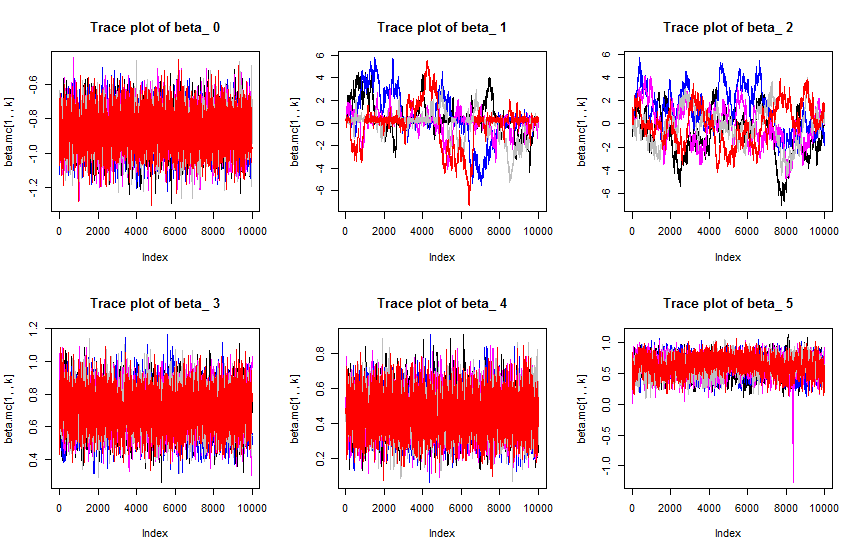
\includegraphics[width=13cm,height=13cm,keepaspectratio]{./images/Prob31}}
\centerline{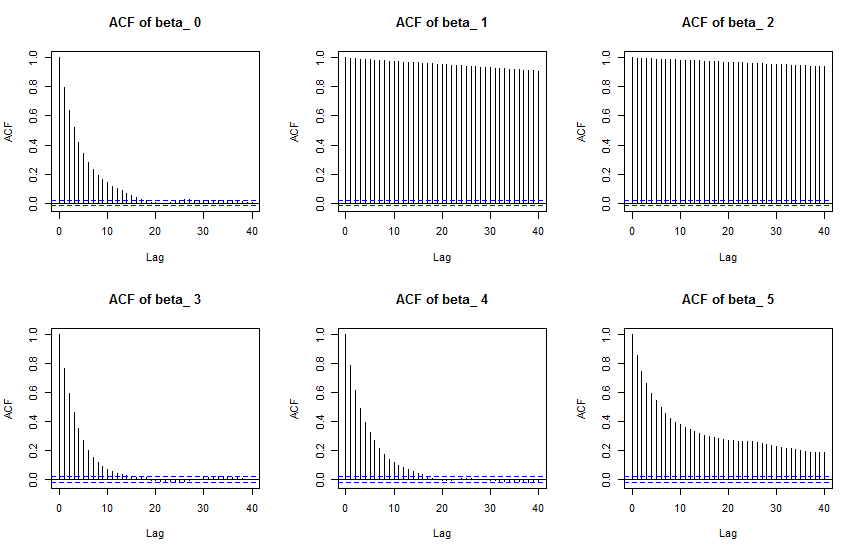
\includegraphics[width=13cm,height=13cm,keepaspectratio]{./images/Prob32}}
\text{}
\\\
\textbf{Part b}\\
We approximated the posterior probability of the top 5 most frequently occurring values of $\gamma$ in the table below. The MCMC estimates of these posterior probabilities are rather accurate,because we ran 10,000 simulations. 

\begin{center}
	\captionof{table}{Top 5 most frequently occurring values for $\gamma$}
  \begin{tabular}{ |c|c|c|c|c|c| }
  \hline
  $\gamma$ & (0,0,1,1,1) & (1,0,1,1,1) & (0,1,1,1,1) & (1,1,1,1,1) & (1,0,0,1,1)  \\ 
  \hline
  Probability & 0.58200 & 0.37315 & 0.02325 & 0.02110 & 0.00015\\ 
  \hline
  \end{tabular}
\end{center}
\text{}
\\\
\textbf{Part c}\\
 We plotted the posterior densities/histograms for each of the $\beta_j \gamma_j$ and calculated their posterior means (Table 2 below). The $Pr(\gamma_j=1|x,y)$ are also given below in Table 3. These results are in accordance with what we calculated in the previous parts. 
\begin{center}
	\captionof{table}{Posterior Means for $\beta_j \gamma_j$}
  \begin{tabular}{ |c|c|c|c|c|c| }
  \hline
  $j$ & 1 & 2 & 3 & 4 & 5  \\ 
  \hline
  Posterior Mean & 0.109 & 0.001 & 0.695 & 0.456 & 0.62\\ 
  \hline
  \end{tabular}
  
  	\captionof{table}{Simulated $Pr(\gamma_j=1|x,y)$}
  \begin{tabular}{ |c|c|c|c|c|c| }
  \hline
  $j$ & 1 & 2 & 3 & 4 & 5  \\ 
  \hline
  $Pr(\gamma_j=1|x,y)$ & 0.3945 & 0.04445 & 0.99965 & 0.99975 &  0.99975\\ 
  \hline
  \end{tabular}
\end{center}
\centerline{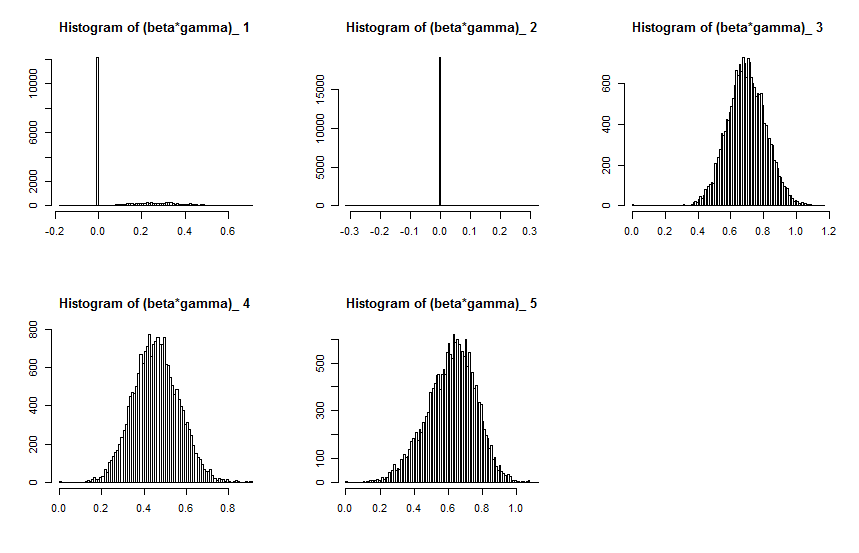
\includegraphics[width=13cm,height=13cm,keepaspectratio]{./images/Prob33}}

\section*{Problem 4}
\textbf{Part 1}
$$
p(\theta_{1}|\theta_{2},\ y)\ =\frac{p(\theta_{1},\theta_{2},y)}{p(\theta_{2},y)}
=\frac{p(y|\theta_{1},\theta_{2})p(\theta_{1},\theta_{2})}{p(y|\theta_{2})p(\theta_{2})}
=\frac{p(y|\theta_{1},\theta_{2})p(\theta_{1})p(\theta_{2})}{p(y|\theta_{2})p(\theta_{2})}
$$
$$
=\frac{p(y|\theta_{1},\theta_{2})p(\theta_{1})}{p(y|\theta_{2})}
\propto\ p(y|\theta_{1},\ \theta_{2})p(\theta_{1})
$$
$$=\frac{1}{2\pi b_1}\exp(-\frac{1}{2}(y-(\theta_{1}+\theta_{2}))^{2})exp(-\frac{1}{2b_{1}^{2}}(\theta_{1}-a_{1})^{2})$$
$$
\propto\ exp(-\frac{1}{2}[y^{2}-2y(\theta_{1}+\theta_{2})+(\theta_{1}+\theta_{2})^{2}])exp(-\frac{1}{2b_{1}^{2}}(\theta_{1}^{2}-2a_{1}\theta_{1}+a_{1}^{2}))
$$
$$
=\ exp(-\frac{1}{2}[(1+\frac{1}{b_{1}^{2}})\theta_{1}^{2}-2(y-\theta_{2}+\frac{a_{1}}{b_{1}^{2}})\theta_{1}+(y^{2}-2y\theta_{2}+\theta_{2}^{2}+\frac{a_{1}^{2}}{b_{1}^{2}})])
$$
$$\sim Normal(\displaystyle \theta_{1};\frac{y-\theta_{2}+\frac{a_{1}}{b_{1}^{2}}}{1+\frac{1}{b_{1}^{2}}},\frac{1}{1+\frac{1}{b_{1}^{2}}})
$$
The other conditional distribution can be derived similarly:
$$
p(\theta_{2}|\theta_{1},y) 
\sim Normal(\displaystyle \theta_{2};\frac{y-\theta_{1}+\frac{a_{2}}{b_{2}^{2}}}{1+\frac{1}{b_{2}^{2}}},\ \frac{1}{1+\frac{1}{b_{2}^{2}}})$$
\textbf{Part 2}\\
\\\
First observe that $p(y|\theta_1) \sim Normal(\theta_1+a_2,b_2^2+1)$. Then we compute:\\
$$
p(\theta_{1}|y) \propto p(y|\theta_1)p(\theta_1)
\propto exp(-\frac{1}{2}[\frac{(y-(\theta_1+a_2))^2}{b_2^2+1}])exp(-\frac{1}{2}[\frac{(\theta_1-a_1)^2}{b_1^2}])$$
$$
= exp(-\frac{1}{2}[\frac{(y^2-2y(\theta_1+a_2)+(\theta_1+a_2)^2)}{b_2^2+1}+\frac{\theta_1^2-2\theta_1 a_1+a_1^2}{b_1^2}])
$$
$$
\sim Normal(\frac{a_{1}+b_{1}^{2}y+a_{1}b_{2}^{2}-a_{2}b_{1}^{2}}{1+b_{1}^{2}+b_{2}^{2}}, \frac{b_{1}^{2}(1+b_{2}^{2})}{1+b_{1}^{2}+b_{2}^{2}})
$$
Similarly, we compute \\
$$ p(\theta_{2}|y) \sim Normal(\frac{a_{2}+b_{2}^{2}y+a_{2}b_{1}^{2}-a_{1}b_{2}^{2}}{1+b_{1}^{2}+b_{2}^{2}}, \frac{b_{2}^{2}(1+b_{1}^{2})}{1+b_{1}^{2}+b_{2}^{2}})$$
The data do update the prior distributions for these parameters.\\
\textbf{Part 3}\\
Using the conditional distributions derived in part 1 to implement the Gibbs sampler here. We started our chains near our prior mean, at 45. As we can see from the trace plots below, for both 100 and 1000 iterations, we do not have convergence for $\theta_1$ or $\theta_2$ but we do have convergence for $\mu=\theta_1+\theta_2$,as it centers around 0. After deleting a burn-in period of $\frac{t}{5}$, the estimated posterior mean for $\mu$ is 0.0275 for 100 iterations and is 0.00919 for 1000 iterations. \\
Below are the simulation results for 100 iterations:\\
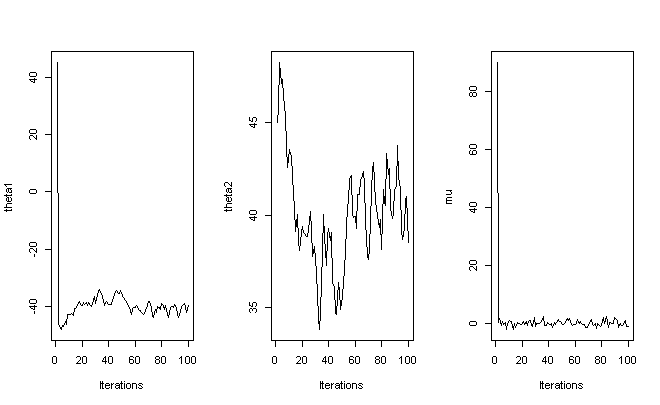
\includegraphics[width=13cm,height=13cm,keepaspectratio]{./images/p1c_100}\\
Below are the simulation results for 1000 iterations:\\
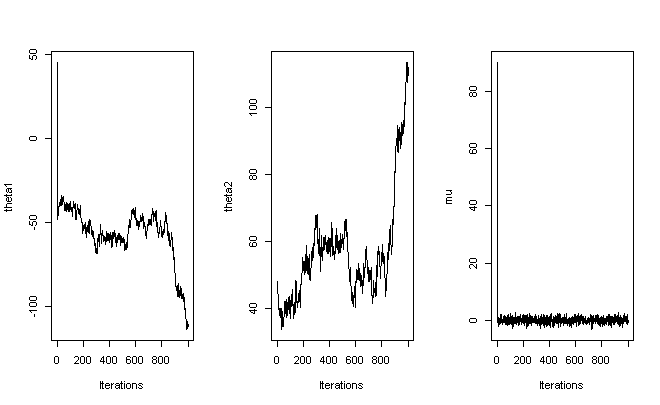
\includegraphics[width=13cm,height=13cm,keepaspectratio]{./images/p1c_1000}\\
R Code attached at end of document
\text{}\\
\\\
\textbf{Part 4}\\
Using the same code, we repeat the above process with different priors, letting $a_1$ and $a_2$ stay the same but changing $b_1=b_2=10$ As we can see from the trace plots below, $\theta_1$ and $\theta_2$ still do not converge but $\mu$ still converges, centered around 0. After deleting a burn-in period of $\frac{t}{5}$, the estimated posterior mean for $\mu$ is 0.395 for 100 iterations and is 0.475 for 1000 iterations. These are higher than the posterior means that we got in part c. \\
Below are the simulation results for 100 iterations:\\
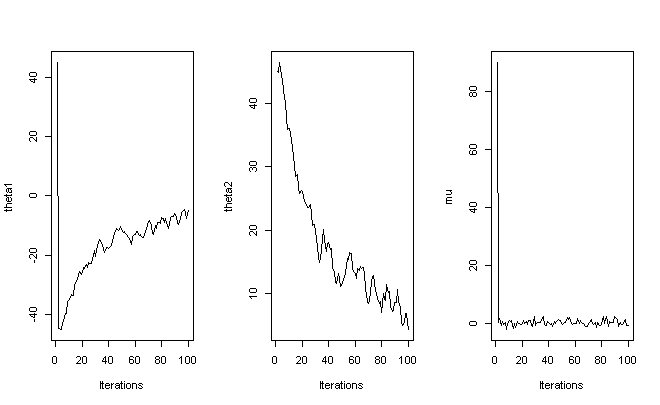
\includegraphics[width=13cm,height=13cm,keepaspectratio]{./images/p1d_100.png}\\
Below are the simulation results for 1000 iterations:\\
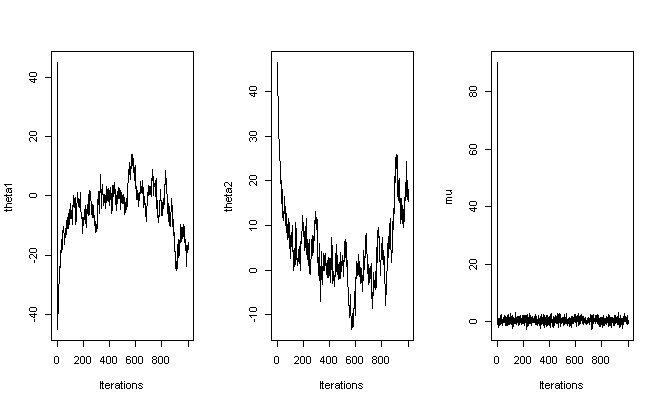
\includegraphics[width=13cm,height=13cm,keepaspectratio]{./images/p1d_1000.png}\\
R Code attached at end of document.

\section*{Problem 5}
\textbf{Part 1}\\
The joint posterior distribution of $\theta,\lambda,b_1,b_2$ is:\\
$$p(\theta,\lambda,b_1,b_2|y_1,...,y_n)\propto \prod_{i=1}^{k}p(y_i|\theta) \prod_{i=k+1}^{n}p(y_i|\lambda)]p(\theta|b_1)p(b_1)p(\lambda|b_2)p(b_2)$$
We can calculate the full conditional distribution for $\theta$:\\
$ p(\theta|rest)\propto[\prod_{i=1}^{k}p(y_i|\theta)]p(\theta|b_1) $\\
$\propto exp(-k\theta)\theta^{\sum_{i=1}^{k}y_i}\theta^{a_1-1}exp(-\frac{\theta}{b_1})  \propto \theta^{a_1+\sum_{i=1}^{k}y_i-1}exp(-\dfrac{\theta}{\frac{b_1}{1+b_1k}}) $
$\propto Gamma(a_1+\sum_{i=1}^{k}y_i,\frac{b_1}{1+b_1k})$\\
Therefore, we have:\\
$$\theta|rest \sim Gamma(a_1+\sum_{i=1}^{k}y_i,\frac{b_1}{1+b_1k})=Gamma(125.5,\frac{b_1}{1+b_1k})$$
We can also calculate the full conditional distribution for $\lambda$:\\
$ p(\lambda|rest) \propto [\prod_{i=k+1}^{n}p(y_i|\lambda)]p(\lambda|b_2)$\\
$ \propto exp(-(n-k)\lambda)\lambda^{\sum_{i=k+1}^{n}y_i}\lambda^{a_2-1}exp(-\frac{\lambda}{b_2}) \propto \theta^{a_2+\sum_{i=k+1}^{n}y_i-1}exp[-\dfrac{\lambda}{\frac{b_2}{1+b_2(n-k)}}] $\\
$ \propto Gamma(a_2+\sum_{i=k+1}^{n}y_i,\frac{b_2}{1+b_2(n-k)}) $\\
So using the data, we have:\\
$$ \lambda|rest \sim Gamma(a_2+\sum_{i=k+1}^{n}y_i,\frac{b_2}{1+b_2(n-k)}) = Gamma(66.5,\frac{b_2}{1+b_2(n-k)}) $$
R cod attached. \\
\\\
\textbf{Part 2}\\
The full conditional distributions for $b_1,b_2$ are the following:\\
$p(b_1|rest)\propto p(\theta|b_1)p(b_1)\propto b_1^{-a_1}exp(-\theta/b_1)b_1^{-(c_1+1)}exp(-\frac{1}{d_1b_1})\propto Inv-Gamma(a_1+c_1,\frac{d_1}{1+d_1\theta})$
$p(b_2|rest)\propto p(\lambda|b_2)p(b_2)\propto b_2^{-a_2}exp(-\lambda/b_2)b_2^{-(c_2+1)}exp(-\frac{1}{d_2b_2})\propto Inv-Gamma(a_2+c_2,\frac{d_2}{1+d_2\lambda})$
So using our given values for $a_i$ and $c_i$,\\
$$p(b_1|rest) \sim IG(a_1+c_1,\frac{d_1}{1+d_1\theta})=IG(1.5,\frac{1}{1+\theta})$$
$$p(b_2|rest) \sim IG(a_2+c_2,\frac{d_2}{1+d_2\lambda})=IG(1.5,\frac{1}{1+\lambda})$$
Please refer to the R code attached. The summary of the posterior samples is given in the table below. The posterior histogram and estimated kernel densities are given in the plots below. Additionally, the trace and acf plots for $\lambda, \theta, \frac{1}{b_1}$, and $\frac{1}{b_2}$ are given below. We can see that the ACF cuts off quickly for all of our parameters, which indicates convergence in the MCMC method. The trace plots also point towards this. 
\begin{center}
  \begin{tabular}{ |c|c|c|c|c| }
  \hline
  Parameter & Mean & Standard Deviation & Lower 2.5\% quantiles & Upper 2.5\% quantiles  \\ 
  $\theta$ & 3.109026 & 0.2780253 & 2.585145 & 3.676767 \\ 
  $\lambda$ & 0.9135259 & 0.1125701 & 0.7069611 & 1.1466074 \\
  $R$ & 3.455759 & 0.532644 & 2.536974 & 4.620163 \\
  \hline
  \end{tabular}
  \end{center}
  
\centerline{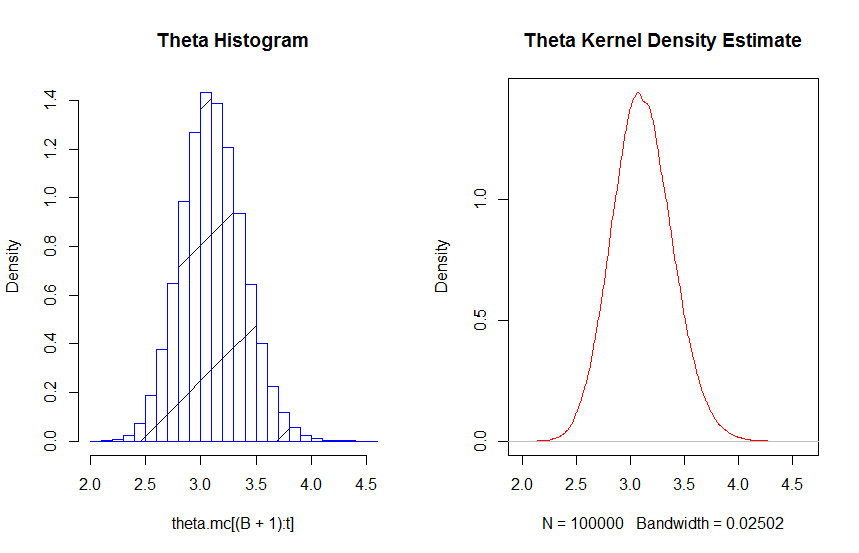
\includegraphics[width=13cm,height=13cm,keepaspectratio]{./images/21}}
\centerline{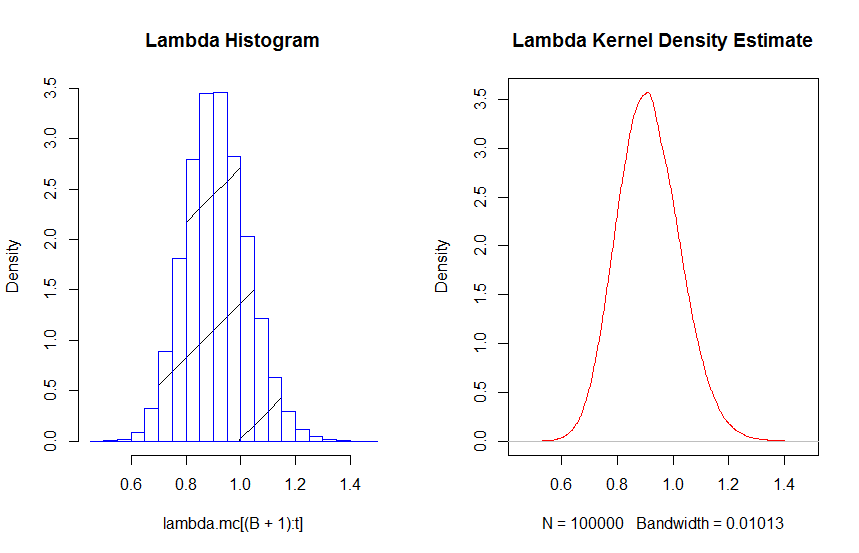
\includegraphics[width=13cm,height=13cm,keepaspectratio]{./images/22}}\centerline{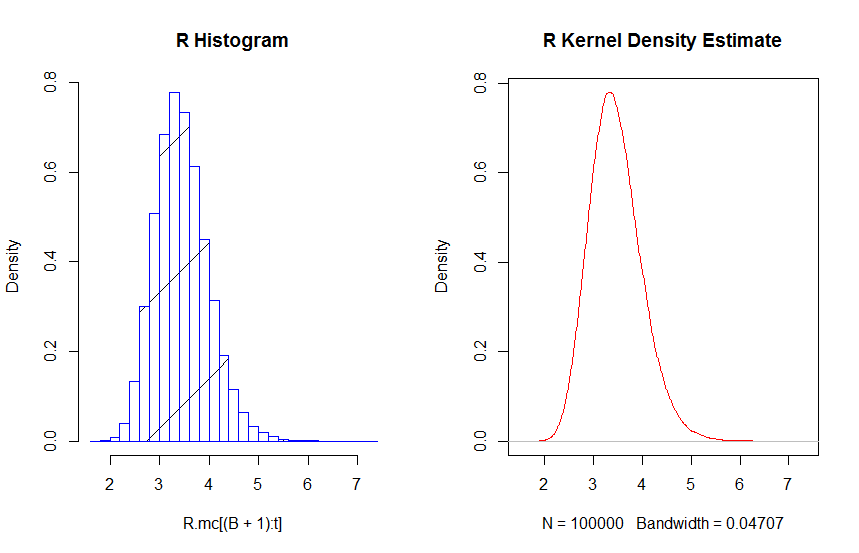
\includegraphics[width=13cm,height=13cm,keepaspectratio]{./images/23}}
\centerline{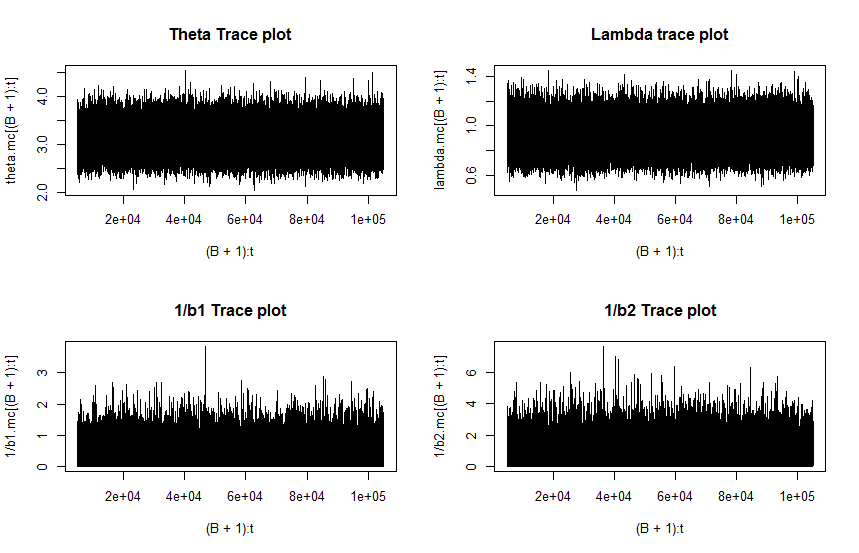
\includegraphics[width=13cm,height=13cm,keepaspectratio]{./images/24}}
\centerline{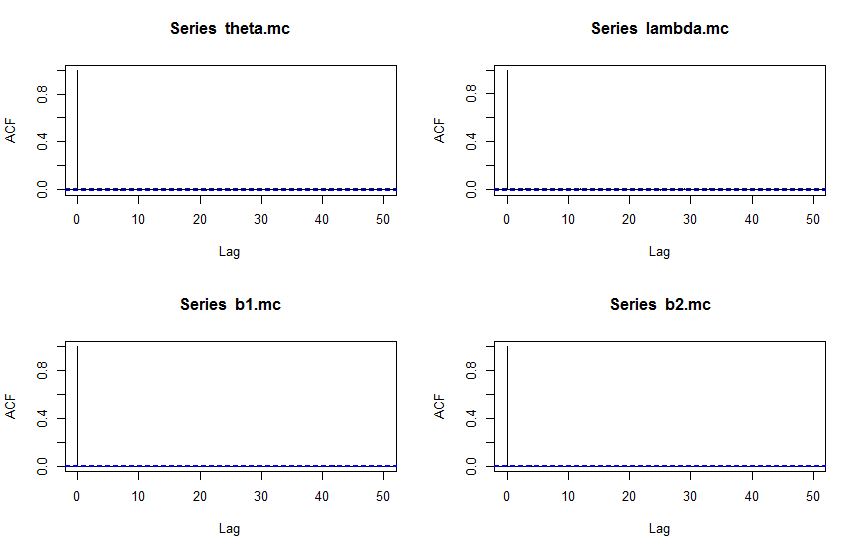
\includegraphics[width=13cm,height=13cm,keepaspectratio]{./images/25}}
\text{}\\
\\\
\textbf{Part 3}\\
First we need to derive the full conditional distribution for k:\\
$$p(k|rest)\propto [\prod_{i=1}^{k}p(y_i|\theta)][\prod_{i=k+1}^{n}p(y_i|\lambda)]p(k)\propto exp(-\theta k)\theta^{\sum_{i=1}^{k}y_i}exp(-\lambda(n-k))\lambda^{\sum_{i=k+1}^{n}y_i} $$
Since this conditional distribution isn't closed-form, we can use Metropolis Hastings as an MCMC method. Please refer to attached R code. A summary of the posterior of R and other parameters is given below. The trace, acf, and posterior density plots for k are given below. The posterior histogram and estimated kernel densities for R are also given below. We can see there is no significant changes to the posterior of R when using an unknown k except for a slight increase in the standard deviation of R.

\begin{center}
  \begin{tabular}{ |c|c|c|c|c| }
  \hline
  Parameter & Mean & Standard Deviation & Lower 2.5\% quantiles & Upper 2.5\% quantiles  \\ 
  $R$ & 3.510614 & 0.635233 & 2.439432 & 4.927623 \\
  $k$ & 39.99012 & 2.382276 & 36 & 46 \\
  $b_1$ & 6.428182 &  97.35294 &  0.6474449 & 28.7964318  \\
  $b_2$ &  1.815688 & 13.99343 & 0.1903916 & 8.4587874 \\
  \hline
  \end{tabular}
  \end{center}
  
\centerline{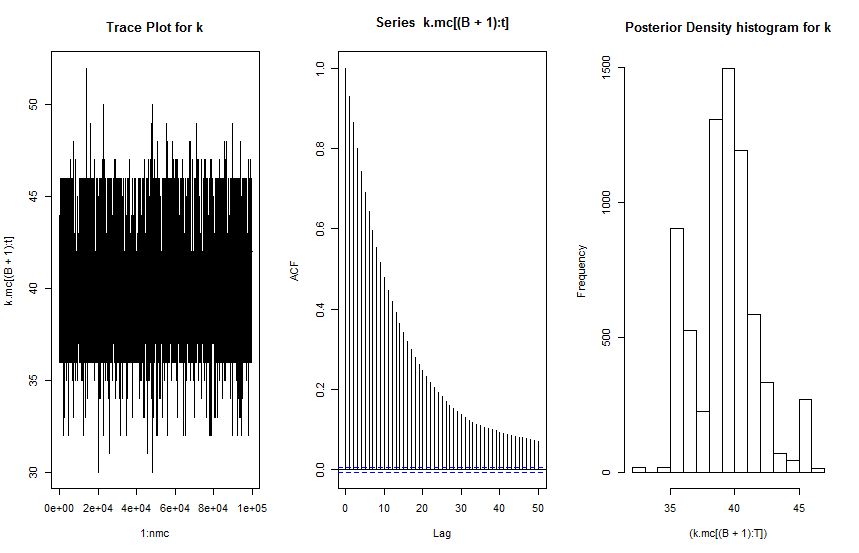
\includegraphics[width=13cm,height=13cm,keepaspectratio]{./images/31}}
\centerline{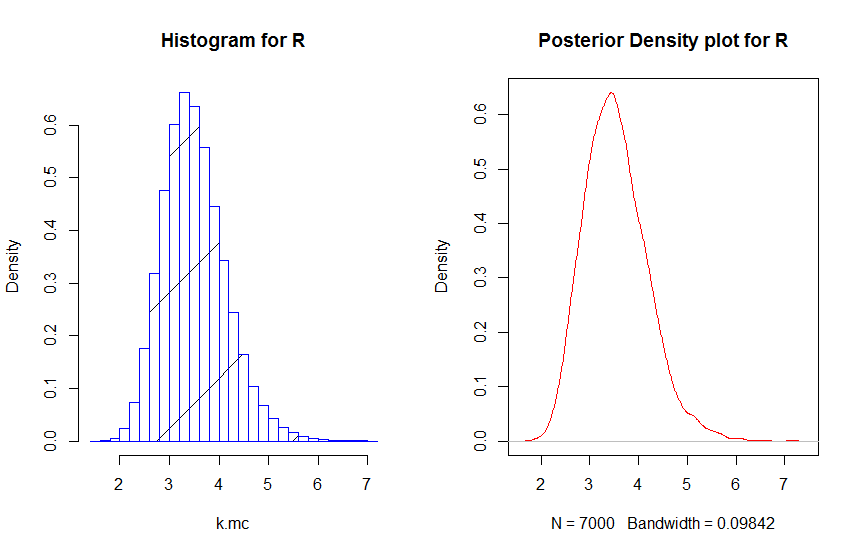
\includegraphics[width=13cm,height=13cm,keepaspectratio]{./images/32}}
\text{}\\
\\\
\textbf{Part 4} \\
We ran Metropolis-Hastings using the priors given to us, and plotted the posterior densities below. Please refer to R code. We can see from the densities and the summary table below that there are no significant changes to the posterior distributions of R and k (comparing with part 3). However, the mean and standard deviation of $b_1$ and $b_2$ increased from those in part 3 due to the change in the priors and hyperparameters. 

\begin{center}
  \begin{tabular}{ |c|c|c|c|c| }
  \hline
  Parameter & Mean & Standard Deviation & Lower 2.5\% quantiles & Upper 2.5\% quantiles  \\ 
  $R$ & 3.48755 & 0.6322124 & 2.414312 & 4.880537 \\
  $k$ & 39.84117 & 2.439205 & 36 & 46 \\
  $b_1$ & 67.47563 &  76.77382 &  3.197285  & 279.340797  \\
  $b_2$ &  59.59499 & 73.61156 & 1.46222 & 267.97947 \\
  \hline
  \end{tabular}
  \end{center}
\centerline{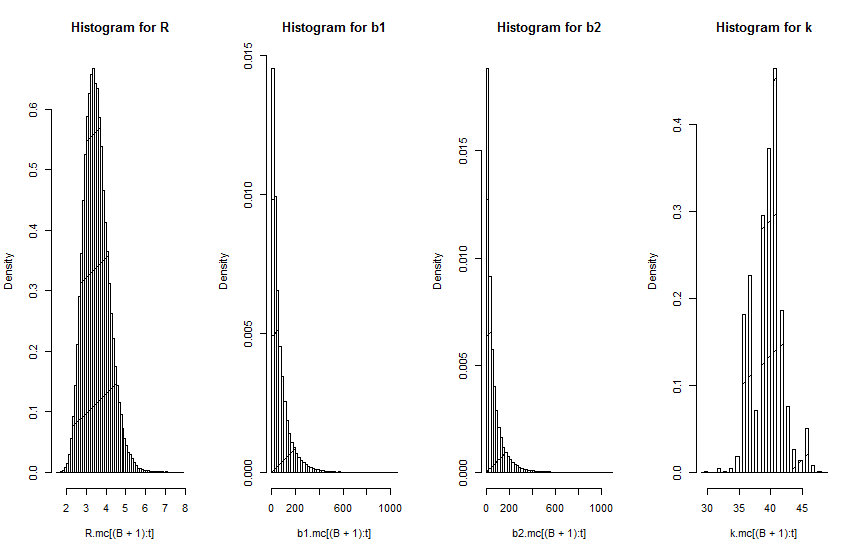
\includegraphics[width=17cm,height=17cm,keepaspectratio]{./images/hist}}
\text{}\\
\\\
\textbf{R Code} 
\lstset{backgroundcolor=\color{light-gray}, frame=single, basicstyle = \ttfamily\small}
\begin{lstlisting}[language=R]
#Problem 3
library(data.table)
library(mvtnorm)

temp <- read.table("azdiabetes.dat",header=TRUE)
temp$diabetes <- array(1*(temp$diabetes=='Yes'))
temp[c('npreg','bp','bmi','ped','age')] <- apply(temp[c('npreg','bp','bmi','ped','age')], 2, function(x) (x - mean(x)) / sd(x))
X <- as.matrix( temp[c('npreg','bp','bmi','ped','age')] )
X <- cbind(1, X)
y <- temp$diabetes
int <- function(x){
  int <- rnorm(n=1, mean=x, sd=.75)
  if(int>=0.5){
    num <- 1
  } else {
    num <- 0
  }
  return(num)
}

loglike <- function(y,beta,gamma.mc,X){ 
  xbeta <- X%*%(beta*c(1,gamma.mc))
  like   <- sum(dbinom(y, 1, (exp(xbeta)/(1+exp(xbeta))), log = TRUE))
  return(like)
}
logprior <- function(beta.mc) {
  return(dmvnorm(beta.mc, mean = c(0,0,0,0,0,0), 
                 sigma = diag(c(16, 4, 4, 4, 4, 4)), log = TRUE))
}
gl.new <- glm(diabetes ~ npreg + bp + bmi + ped + age
             , data = temp, family = binomial)
tau <- c(1,1,1,1,1,1)*summary(gl.new)$coefficients[,2]

p <- 6
nmc <- 10000
chains <- 5
beta.mc <- array(NA, dim = c(chains, nmc, p))
for (i in 1:chains) {
  beta.mc[i, 1, ] <- gl.new$coefficients
}
gamma.mc <- array(NA, dim = c(chains, nmc, p-1))
for (i in 1:chains) {
  gamma.mc[i, 1, ] <- rep(0,(p-1))
}
for (i in 1:chains) {
  for (j in 2:nmc) {
    beta.mc[i, j, ] <- beta.mc[i, j - 1, ]
    gamma.mc[i, j, ] <- gamma.mc[i, j - 1, ]
    
    for (k in 1:p) {
      current_betas <- beta.mc[i, j, ]
      proposed_betas <- current_betas
      proposed_betas[k] <- rnorm(1, beta.mc[i, j-1, k], tau[k])
      
      log_AR <- loglike(y = y, beta = proposed_betas, gamma.mc = gamma.mc[i, (j-1), ], X = X) + 
        logprior(beta.mc = proposed_betas) -
        loglike(y = y, beta = current_betas, gamma.mc = gamma.mc[i, (j-1), ], X = X) -
        logprior(beta.mc = current_betas)
      U=runif(1)
      if (U < exp(log_AR)) {
        beta.mc[i, j, k] <- proposed_betas[k]
      }
    }
    for(l in 1:(p-1)){
      current_gamma <- gamma.mc[i, j, ]
      proposed_gamma <- current_gamma
      proposed_gamma[l] <- int(gamma.mc[i, (j-1), l])
      log_AR <- loglike(y = y, beta = beta.mc[i, j, ], gamma.mc = proposed_gamma, X = X) -
        loglike(y = y, beta = beta.mc[i, j, ], gamma.mc = current_gamma, X = X) 
      if (log(runif(1)) < log_AR) {
        gamma.mc[i, j, l] <- proposed_gamma[l]
      }
    }
  }
} 
#part a trace and acf
par(mfrow=c(2,3))
for (k in 1:6){
  plot(beta.mc[1, , k], type = 'l',
       ylim = range(beta.mc[ , , k]), main = paste('Trace plot of beta_',k-1))
  for (i in 2:chains) {
    lines(beta.mc[i, , k], col = (2*i))
  }
}

par(mfrow=c(2,3))
for (pp in 1:6){
  acf(beta.mc[1,,pp],main = paste('ACF of beta_',pp-1))
}

gamma_set <- apply(rbind(gamma.mc[1,,],gamma.mc[2,,]),1, function(x) paste(x, collapse = ''))
comb <- array(unique(gamma_set))
count <- apply(comb, 1, function(x) length(grep(x, gamma_set)))
Prob <- count/length(gamma_set)
table <- data.frame(comb, count, Prob)
table[order(-count),] 
beta.gamma <- cbind(1,rbind(gamma.mc[1,,],gamma.mc[2,,]))*rbind(beta.mc[1,,],beta.mc[2,,])
means <- apply(beta.gamma, 2, mean)
beta_gamma <- array(NA, 6)
for (i in 1:6){
  beta_gamma[i] <- paste("(beta*gamma)_",i-1)
}
coeff <- round(means,3)
data.frame(cbind(beta_gamma, coeff))
Prob_gamma <- apply(rbind(gamma.mc[1,,],gamma.mc[2,,]), 2, mean)
gamma_i <- array(NA, 5)
for (i in 1:5){
  gamma_i[i] <- paste("gamma_",i)
}
#Part c hist
data.frame(cbind(gamma_i, Prob_gamma))
par(mfrow=c(2,3))
for (i in 2:6){
  hist(beta.gamma[,i], breaks = 100,
       ylab = '', xlab = '',
       main = paste("Histogram of (beta*gamma)_",i-1))
}

# Problem 4 Part 3
> a1 <- 50
> a2 <- 50
> b1 <- 1000
> b2 <- 1000
> t <- 1000;
> set.seed(1);
> theta1 <- numeric(t)
> theta2 <- numeric(t)
> theta1[1] <- 45
> theta2[1] <- 45
> n <- 1
> for(i in 2:t) {
+   theta1[i] <- rnorm(1, (-n*theta2[i-1]+a1/b1^2)/(n+1/b1^2), sqrt(1/((n+1/b1^2))))
+   theta2[i] <- rnorm(1, (-n*theta1[i]+a2/b2^2)/(n+1/b2^2), sqrt(1/((n+1/b2^2))))
+ }
> par(mfrow = c(1, 3))
> plot(theta1, type = 'l', xlab = "Iterations", ylab = "theta1")
> plot(theta2, type = 'l', xlab = "Iterations", ylab = "theta2")
> plot(theta1+theta2, type = 'l', xlab = "Iterations", ylab = "mu")
> mean(theta1[(t/5+1):t]+theta2[(t/5+1):t])
[1] 0.009187082

> # Problem 4 Part 4
> a1 <- 50
> a2 <- 50
> b1 <- 10
> b2 <- 10
> t <- 1000;
> set.seed(1);
> theta1 <- numeric(t)
> theta2 <- numeric(t)
> theta1[1] <- 45
> theta2[1] <- 45
> n <- 1
> for(i in 2:t) {
+   theta1[i] <- rnorm(1, (-n*theta2[i-1]+a1/b1^2)/(n+1/b1^2), sqrt(1/((n+1/b1^2))))
+   theta2[i] <- rnorm(1, (-n*theta1[i]+a2/b2^2)/(n+1/b2^2), sqrt(1/((n+1/b2^2))))
+ }
> par(mfrow = c(1, 3))
> plot(theta1, type = 'l', xlab = "Iterations", ylab = "theta1")
> plot(theta2, type = 'l', xlab = "Iterations", ylab = "theta2")
> plot(theta1+theta2, type = 'l', xlab = "Iterations", ylab = "mu")
> mean(theta1[(t/5+1):t]+theta2[(t/5+1):t])
[1] 0.4750674

#Problem 5
data=read.table("coal_data.txt",header=FALSE)
data$V1=data$V1-1850
# part 1
a1 = a2 =0.5
c1 = c2 = 1
d1 = d2 = 1
k = 40
d=data$V2
n=length(d)
d.sum.1=sum(d[1:k]) 
d.sum.2=sum(d[(k+1):n]) 
#################################
# part 2
B=5000 
nmc=100000 
t=B+nmc 
theta.mc=lambda.mc=b1.mc=b2.mc=numeric(t)
theta.mc[1]=mean(d[1:k])
lambda.mc[1]=mean(d[(k+1):n])
b1.mc[1]=b2.mc[1]=1
#Gibbs sampler
for (i in 2:t){
  theta.mc[i]=rgamma(1,shape=a1+sum(d[1:k]),scale=b1.mc[i-1]/(1+b1.mc[i-1]*k))
  lambda.mc[i]=rgamma(1,shape=a2+sum(d[(k+1):n]), scale=b2.mc[i-1]/(1+b2.mc[i-1]*(n-k)))
  b1.mc[i]=1/rgamma(1,shape=a1+c1,scale=d1/(1+d1*theta.mc[i]))
  b2.mc[i]=1/rgamma(1,shape=a2+c2,scale=d2/(1+d2*lambda.mc[i]))
}
R.mc=theta.mc/lambda.mc
#Posterior sample summaries: mean, std dev, quantiles 
mean(theta.mc[(B+1):t])
sd(theta.mc[(B+1):t])
quantile(theta.mc[(B+1):t],probs=c(0.025,0.975))
mean(lambda.mc[(B+1):t])
sd(lambda.mc[(B+1):t])
quantile(lambda.mc[(B+1):t],probs=c(0.025,0.975))
mean(R.mc[(B+1):t])
sd(R.mc[(B+1):t])
quantile(R.mc[(B+1):t],probs=c(0.025,0.975))

#Plot the histograms and Kernel Density estimate
par(mfrow=c(1,2))
hist(theta.mc[(B+1):t],nclass=25,density=TRUE,
     probability = TRUE,border = "blue", main="Theta Histogram")
plot(density(theta.mc[(B+1):t]),type="l",main="Theta Kernel Density Estimate",col="red")


hist(lambda.mc[(B+1):t],nclass=25,density=TRUE,
     probability = TRUE,border = "blue", main="Lambda Histogram")
plot(density(lambda.mc[(B+1):t]),type="l",main="Lambda Kernel Density Estimate",col="red")

hist(R.mc[(B+1):t],nclass=25,density=TRUE,
     probability = TRUE,border = "blue",main="R Histogram")
plot(density(R.mc[(B+1):t]),type="l",main="R Kernel Density Estimate",col="red")


# Plot the trace plots and the autocorrelation plots to check convergence
par(mfrow=c(2,2))
plot((B+1):t,theta.mc[(B+1):t],type="l",main="Theta Trace plot")
plot((B+1):t,lambda.mc[(B+1):t],type="l",main="Lambda trace plot")
plot((B+1):t,1/b1.mc[(B+1):t],type="l",main="1/b1 Trace plot")
plot((B+1):t,1/b2.mc[(B+1):t],type="l",main="1/b2 Trace plot")
acf(theta.mc)
acf(lambda.mc)
acf(b1.mc)
acf(b2.mc)
############################################
# part 3
B=5000
nmc=100000
t=B+nmc
k.mc=numeric(t)
theta.mc=lambda.mc=b1.mc=b2.mc=numeric(t)
theta.mc[1]=mean(d[1:k])
lambda.mc[1]=mean(d[(k+1):n])
b1.mc[1]= 8.292544
b2.mc[1]= 3.849951
k.mc[1]=40
#function to calculate log probability for k
logpk<-function(k,d,theta,lambda){
  logp.theta=-theta*k+log(theta)*sum(d[1:k])
  if (k==n){
    logp.lambda=0
  }else{
    logp.lambda=-lambda*(n-k)+log(lambda)*sum(d[(k+1):n])
    }
  return(logp.theta+logp.lambda)
}
for (i in 2:t){
  theta.mc[i]=rgamma(1,shape=a1+sum(d[1:k]), scale=b1.mc[i-1]/(1+b1.mc[i-1]*k.mc[i-1]))
  lambda.mc[i]=rgamma(1,shape=a2+sum(d[(k+1):n]), scale=b2.mc[i-1]/(1+b2.mc[i-1]*(n-k.mc[i-1])))
  b1.mc[i]=1/rgamma(1,shape=a1+c1, scale=d1/(1+d1*theta.mc[i]))
  b2.mc[i]=1/rgamma(1,shape=a2+c2, scale=d2/(1+d2*lambda.mc[i]))

  k.star=sample.int(n,size=1,replace=TRUE)
  logpk.star=logpk(k.star,d,theta.mc[i],lambda.mc[i])
  logpk.i=logpk(k.mc[i-1],d,theta.mc[i],lambda.mc[i])
  rho=min(c(1,exp(logpk.star-logpk.i)))
  U=runif(1)
  if (U<rho) {
    k.mc[i]=k.star
  }else{
    k.mc[i]=k.mc[i-1]
  }
}
R.mc=theta.mc/lambda.mc
#Plots
par(mfrow=c(1,3))
plot(1:nmc,k.mc[(B+1):t],type="l", main="Trace Plot for k")
acf(k.mc[(B+1):t])
hist((k.mc[(B+1):T]),type="l",main="Posterior Density histogram for k")
par(mfrow=c(1,2))
hist(R.mc[(B+1):t],nclass=30,density=TRUE,probability=TRUE,border="blue",xlab="k.mc",main="Histogram for R")
plot(density(R.mc[(B+1):T]),type="l",col="red",main="Posterior Density plot for R")

mean(R.mc[(B+1):t])
sd(R.mc[(B+1):t])
quantile(R.mc[(B+1):t],probs=c(0.025,0.975))
mean(k.mc[(B+1):t])
sd(k.mc[(B+1):t])
quantile(k.mc[(B+1):t],probs=c(0.025,0.975))
mean(b1.mc[(B+1):t])
sd(b1.mc[(B+1):t])
quantile(b1.mc[(B+1):t],probs=c(0.025,0.975))
mean(b2.mc[(B+1):t])
sd(b2.mc[(B+1):t])
quantile(b2.mc[(B+1):t],probs=c(0.025,0.975))
############################################
# part 4

B=5000
nmc=100000
t=B+nmc
k.mc=rep(NA,t)
c1 = c2 = 1
d1 = d2 = 100
theta.mc=lambda.mc=b1.mc=b2.mc=rep(NA,t)
theta.mc[1]=mean(d[1:k])
lambda.mc[1]=mean(d[(k+1):n])
b1.mc[1]=8
b2.mc[1]=4
k.mc[1]=40
for (i in 2:t){
  theta.mc[i]=rgamma(1,shape=a1+sum(d[1:k]),
                     scale=b1.mc[i-1]/(1+b1.mc[i-1]*k.mc[i-1]))
  lambda.mc[i]=rgamma(1,shape=a2+sum(d[(k+1):n]),
                      scale=b2.mc[i-1]/(1+b2.mc[i-1]*(n-k.mc[i-1])))
  b1.star=rgamma(1,shape=c1,scale=d1)
  MH.ratio=dgamma(theta.mc[i],shape=a1,scale=b1.star)/
    dgamma(theta.mc[i],shape=a1,scale=b1.mc[i-1])
  rho=min(c(1,MH.ratio))
  if (runif(1,min=0,max=1)<rho){
    b1.mc[i]=b1.star
  }else{
    b1.mc[i]=b1.mc[i-1]
  }
  
  b2.star=rgamma(1,shape=c2,scale=d2)
  MH.ratio=dgamma(lambda.mc[i],shape=a2,scale=b2.star)/
    dgamma(lambda.mc[i],shape=a2,scale=b2.mc[i-1])
  rho=min(c(1,MH.ratio))
  if (runif(1,min=0,max=1)<rho){
    b2.mc[i]=b2.star
  }else{
    b2.mc[i]=b2.mc[i-1]
  }
  
  k.star=sample.int(n,size=1,replace=TRUE)
  logpk.star=logpk(k=k.star,d,theta=theta.mc[i],
                    lambda=lambda.mc[i])
  logpk.i=logpk(k=k.mc[i-1],d,theta=theta.mc[i],
                 lambda=lambda.mc[i])
  rho=min(c(1,exp(logpk.star-logpk.i)))
  if (runif(1,min=0,max=1)<rho){
    k.mc[i]=k.star
  }else{
    k.mc[i]=k.mc[i-1]
  }
}

R.mc=theta.mc/lambda.mc
#Plot Histograms
par(mfrow=c(1,4))
hist(R.mc[(B+1):t],nclass=50,probability=TRUE,density=TRUE, main="Histogram for R")
hist(b1.mc[(B+1):t],nclass=50,probability=TRUE,density=TRUE, main="Histogram for b1")
hist(b2.mc[(B+1):t],nclass=50,probability=TRUE,density=TRUE, main="Histogram for b2")
hist(k.mc[(B+1):t],nclass=50,probability=TRUE,density=TRUE,main="Histogram for k")

# Compute posterior sample summary
mean(R.mc[(B+1):t])
sd(R.mc[(B+1):t])
quantile(R.mc[(B+1):t],probs=c(0.025,0.975))
mean(k.mc[(B+1):t])
sd(k.mc[(B+1):t])
quantile(k.mc[(B+1):t],probs=c(0.025,0.975))
mean(b1.mc[(B+1):t])
sd(b1.mc[(B+1):t])
quantile(b1.mc[(B+1):t],probs=c(0.025,0.975))
mean(b2.mc[(B+1):t])
sd(b2.mc[(B+1):t])
quantile(b2.mc[(B+1):t],probs=c(0.025,0.975))
\end{lstlisting} 
\end{document}